\documentclass{standalone}
\usepackage{pgfplots}
\usepackage{pgfplotstable}
\pgfplotsset{compat=1.16}
\usetikzlibrary{matrix,chains,trees,scopes,decorations,arrows.meta,automata,positioning,shadows,3d}


\begin{document}
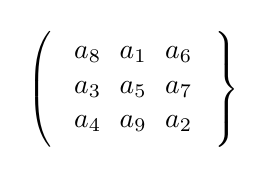
\begin{tikzpicture}
    \matrix [matrix of math nodes,left delimiter=(,right delimiter=\}]
    {
    a_8 & a_1 & a_6 \\
    a_3 & a_5 & a_7 \\
    a_4 & a_9 & a_2 \\
    };
\end{tikzpicture}
\hspace*{2em}
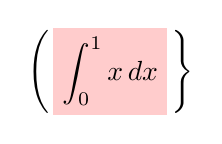
\begin{tikzpicture}
    \node [fill=red!20,left delimiter=(,right delimiter=\}]
    {$\displaystyle\int_0^1 x\,dx$};
\end{tikzpicture}
\hspace*{2em}
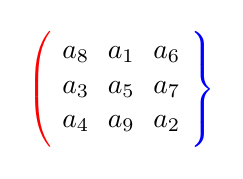
\begin{tikzpicture}
    [every left delimiter/.style={red,xshift=1ex},
    every right delimiter/.style={blue,xshift=-1ex}]
    \matrix [matrix of math nodes,left delimiter=(,right delimiter=\}]
    {
    a_8 & a_1 & a_6 \\
    a_3 & a_5 & a_7 \\
    a_4 & a_9 & a_2 \\
    };
\end{tikzpicture}
\hspace*{2em}
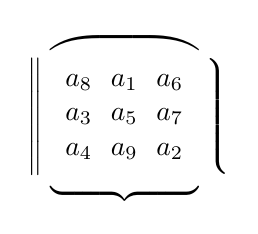
\begin{tikzpicture}
    \matrix [matrix of math nodes,%
    left delimiter=\|,right delimiter=\rmoustache,%
    above delimiter=(,below delimiter=\}]
    {
    a_8 & a_1 & a_6 \\
    a_3 & a_5 & a_7 \\
    a_4 & a_9 & a_2 \\
    };
\end{tikzpicture}
\end{document}
